\documentclass{article}
\usepackage[russian]{babel}
\usepackage[a5paper,top=0.5cm,bottom=2cm,left=1cm,right=1cm,marginparwidth=1.75cm]{geometry}
\usepackage{amsmath}
\usepackage{subfigure}
\usepackage{graphicx}
\usepackage[colorlinks=true, allcolors=blue]{hyperref}
\usepackage{indentfirst}
\usepackage{caption}
\usepackage{multirow}
\usepackage{hhline}
\usepackage{wrapfig}
\usepackage[export]{adjustbox}
\usepackage{esvect}
\usepackage{amsfonts}
\usepackage[dvipsnames]{xcolor}
\usepackage{titlesec}
\usepackage{imakeidx}
\usepackage{nicefrac}
\usepackage{bigints}
\usepackage{xcolor, color, soul}
\sethlcolor{red}

\titleformat*{\section}{\normalsize\bfseries}

\newcommand\ddfrac[2]{\frac{\displaystyle #1}{\displaystyle #2}}
\newcommand{\R}{\mathbb{R}}
\newcommand{\N}{\mathbb{N}}
\newcommand{\bb}{\textbf}
\newcommand{\ii}{\textit}
\newcommand{\x}{\text}
\date{}

\setlength{\abovecaptionskip}{1pt}
\setlength{\belowcaptionskip}{1pt}

\begin{document}
\noindent

\tableofcontents

\newpage
\section{\color{RedViolet}\textbf{Предел последовательности точек в n-мерном евклидовом пространстве. Связь между сходимостью последовательности точек и сходимостью последовательностей их координат. Внутренние, предельные, изолированные точки множества. Открытые и замкнутые множества, их свойства. Внутренность, замыкание и граница множества.}}
\vspace{-0.5cm}
\begin{figure}[h!]
    \centering
    
\includegraphics[width=\textwidth]{1.png}
    \vspace{-1cm}
\end{figure}
\begin{figure}[h!]
    \centering
    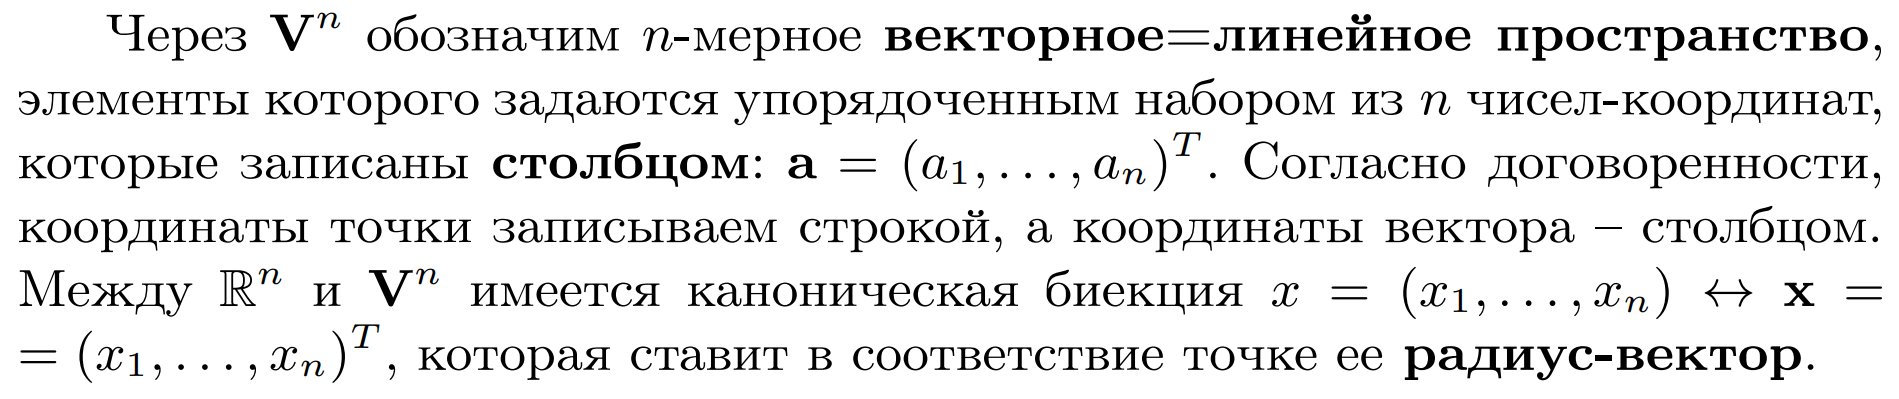
\includegraphics[width=\textwidth]{12.png}
    \vspace{-1cm}
\end{figure}
\begin{figure}[h!]
    \centering
    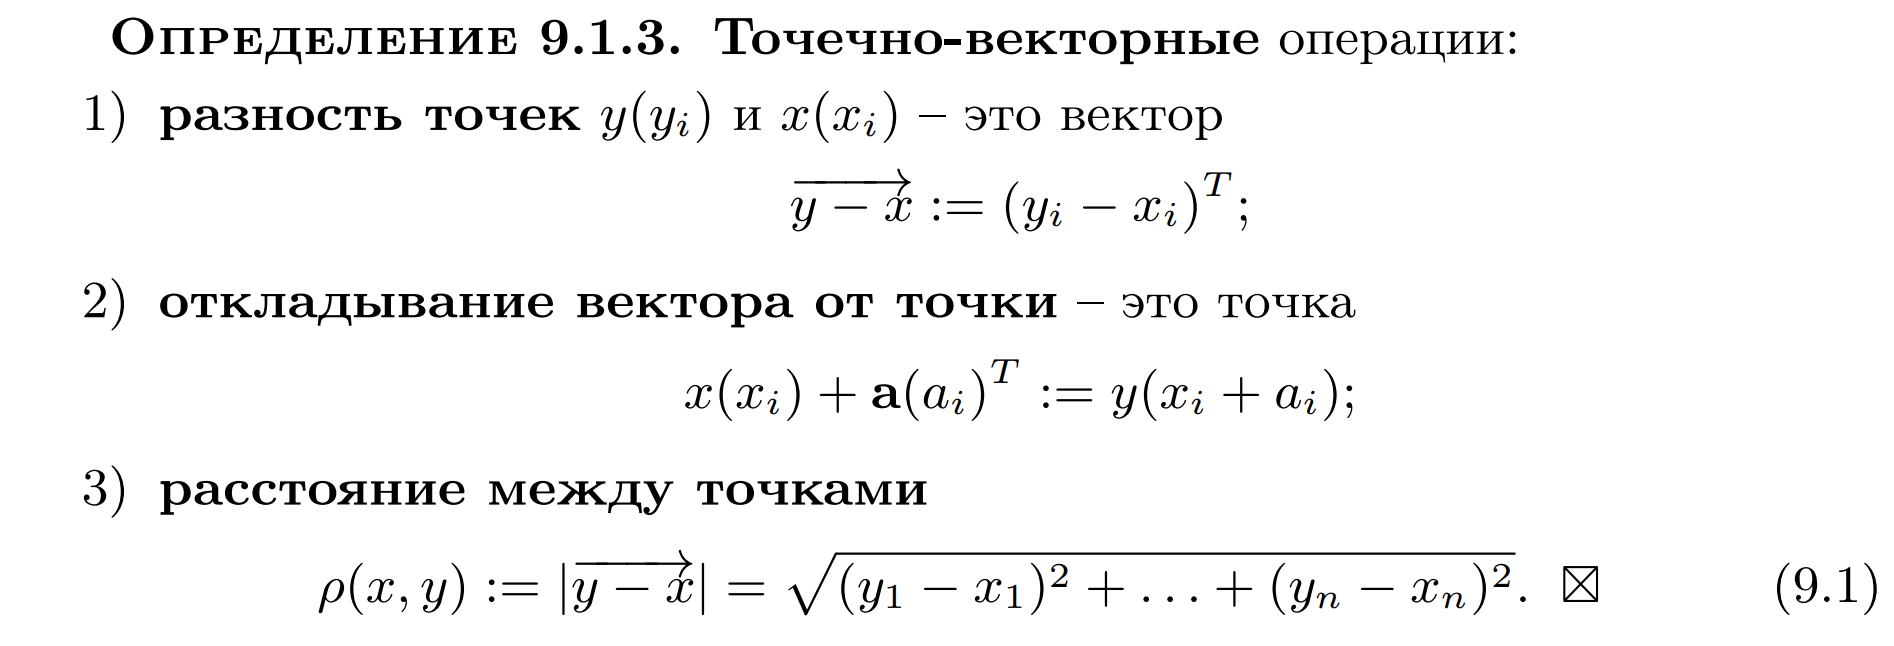
\includegraphics[width=\textwidth]{11.png}
    \vspace{-1cm}
\end{figure}
\begin{figure}[h!]
    \centering
    
\includegraphics[width=\textwidth]{2.png}
    \vspace{-1cm}
\end{figure}
\begin{figure}[h!]
    \centering
    \fbox{
\includegraphics[width=\textwidth]{3.png}}
    \vspace{-1cm}
\end{figure}
\begin{figure}[h!]
    \centering
    \fbox{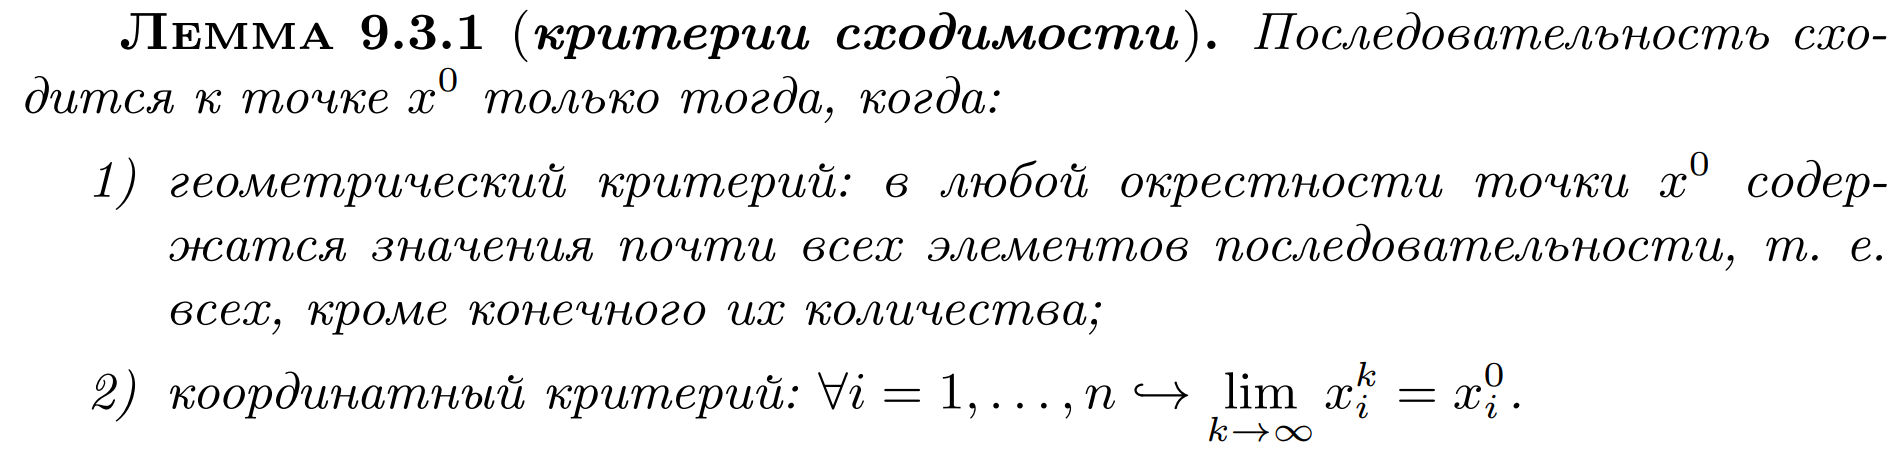
\includegraphics[width=\textwidth]{4.png}}
    \vspace{-1cm}
\end{figure}
\begin{figure}[h!]
    \centering
    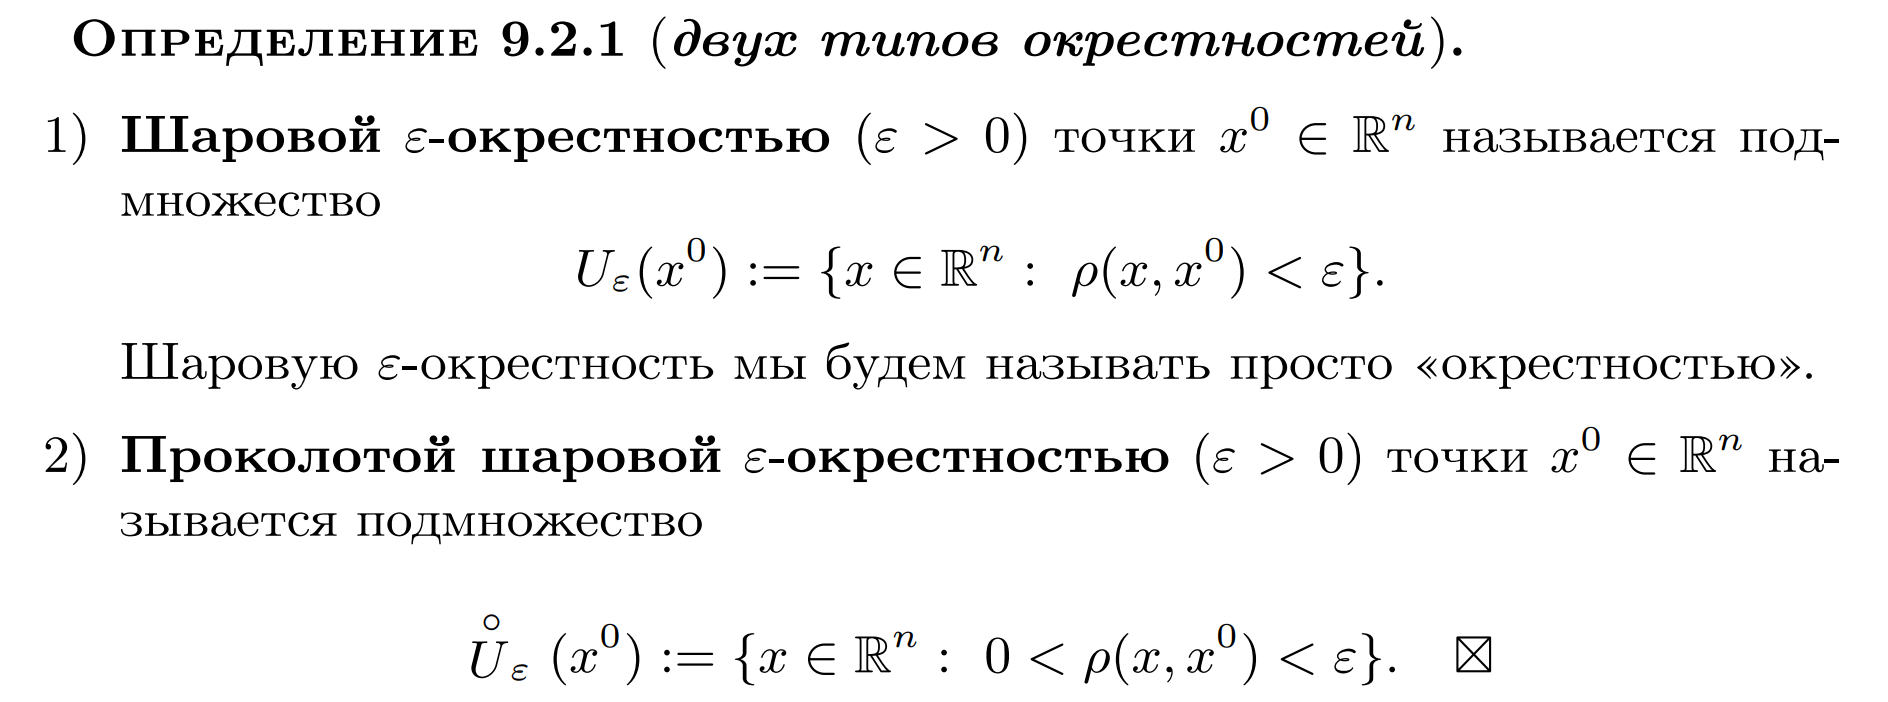
\includegraphics[width=\textwidth]{7.png}
    \vspace{-1cm}
\end{figure}
\newpage
\begin{figure}[h!]
    \centering
    \fbox{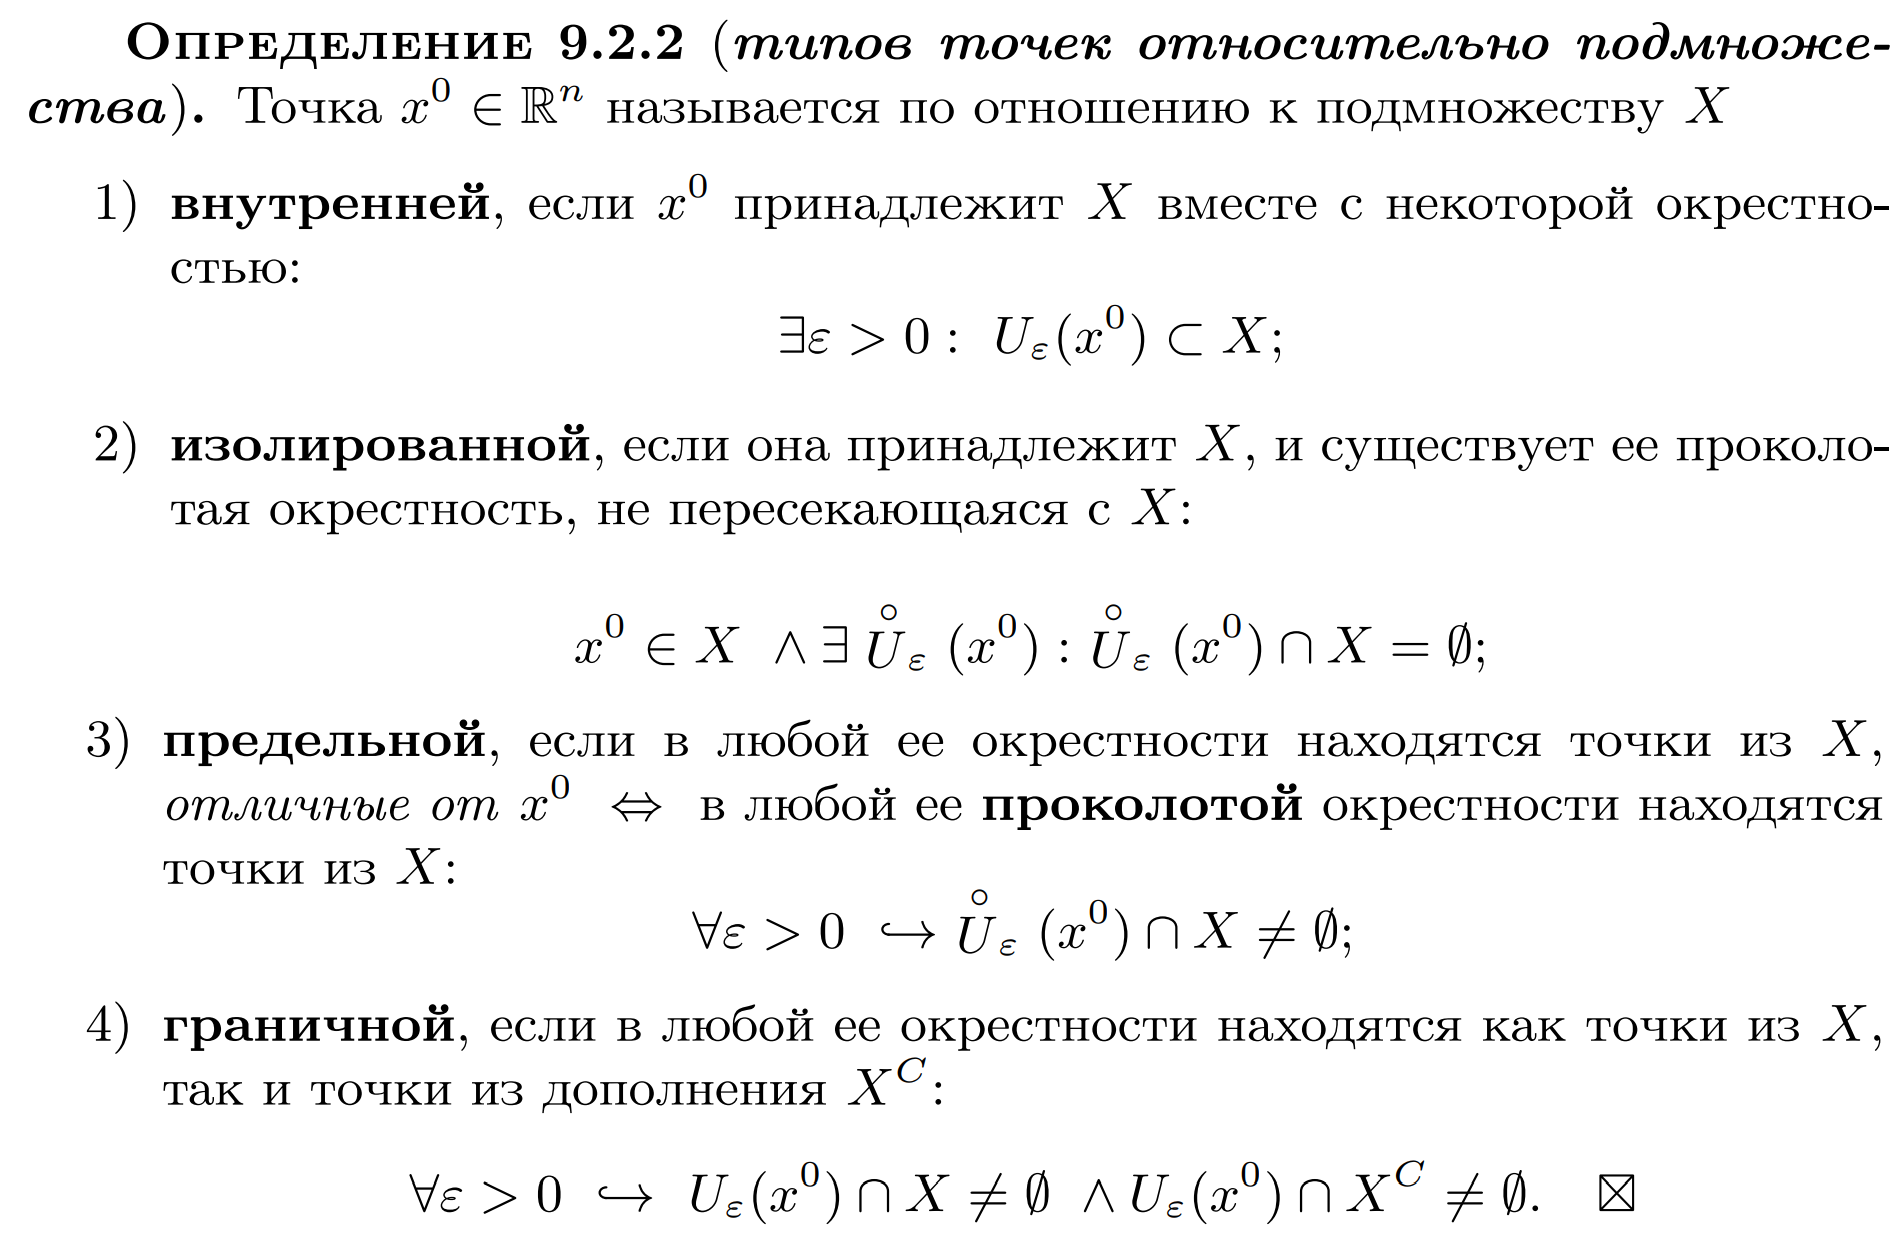
\includegraphics[width=\textwidth]{5.png}}
\end{figure}
{\bfseries\colorbox{lightgray}{Def}} $x_0$ называется точкой прикосновения множества $E$, если в любой её окресности найдутся точки из множества (не проколотой).

Изолированная точка является точкой прикосновения, но не является предельной, любая предельная является изолированной.

Изолированные точки обязательно принадлежат множеству, граничные могут не принадлежать ($(0,1)\cup \{2\}$ и концы $(0,1)$)
\begin{figure}[h!]
    \centering
    
\includegraphics[width=\textwidth]{8.png}
    \vspace{-1cm}
\end{figure}

{\bfseries\colorbox{lightgray}{Def}} (эквивалентное) $x^{0}$ -- предельная точка $E$, если $\exists x^{m} \to x^{(0)}, x^{m}\neq x^{(0)}$.

\newpage

\begin{figure}[h!]
    \centering
    \fbox{
\includegraphics[width=\textwidth]{9.png}}
\end{figure}

{\bfseries\colorbox{lightgray}{Def}} (альтернативные определения замкнутого множества) $M$ -- замкнуто, если оно содержит все свои граничные точки (точки прикосновения), (дополнение $\overline{M}$ открыто)

{\bfseries\colorbox{lightgray}{Def}} \bb{Область} -- открытое, линейно связное множество.

{\bfseries\colorbox{lightgray}{Def}} $E$ -- \bb{линейно связное множество}, если $\forall x_1, x_2 \in E$ можем соединить кривойБ принадлежащей $E$

{\bfseries\colorbox{lightgray}{Def}} \bb{Компакт} -- ограниченное, замкнутое множество.

{\bfseries\colorbox{lightgray}{Def}} $E$ -- ограничено, если $\exists U_\varepsilon(0) : E\subset U_\varepsilon(0)$

\begin{figure}[h!]
    \centering
    \fbox{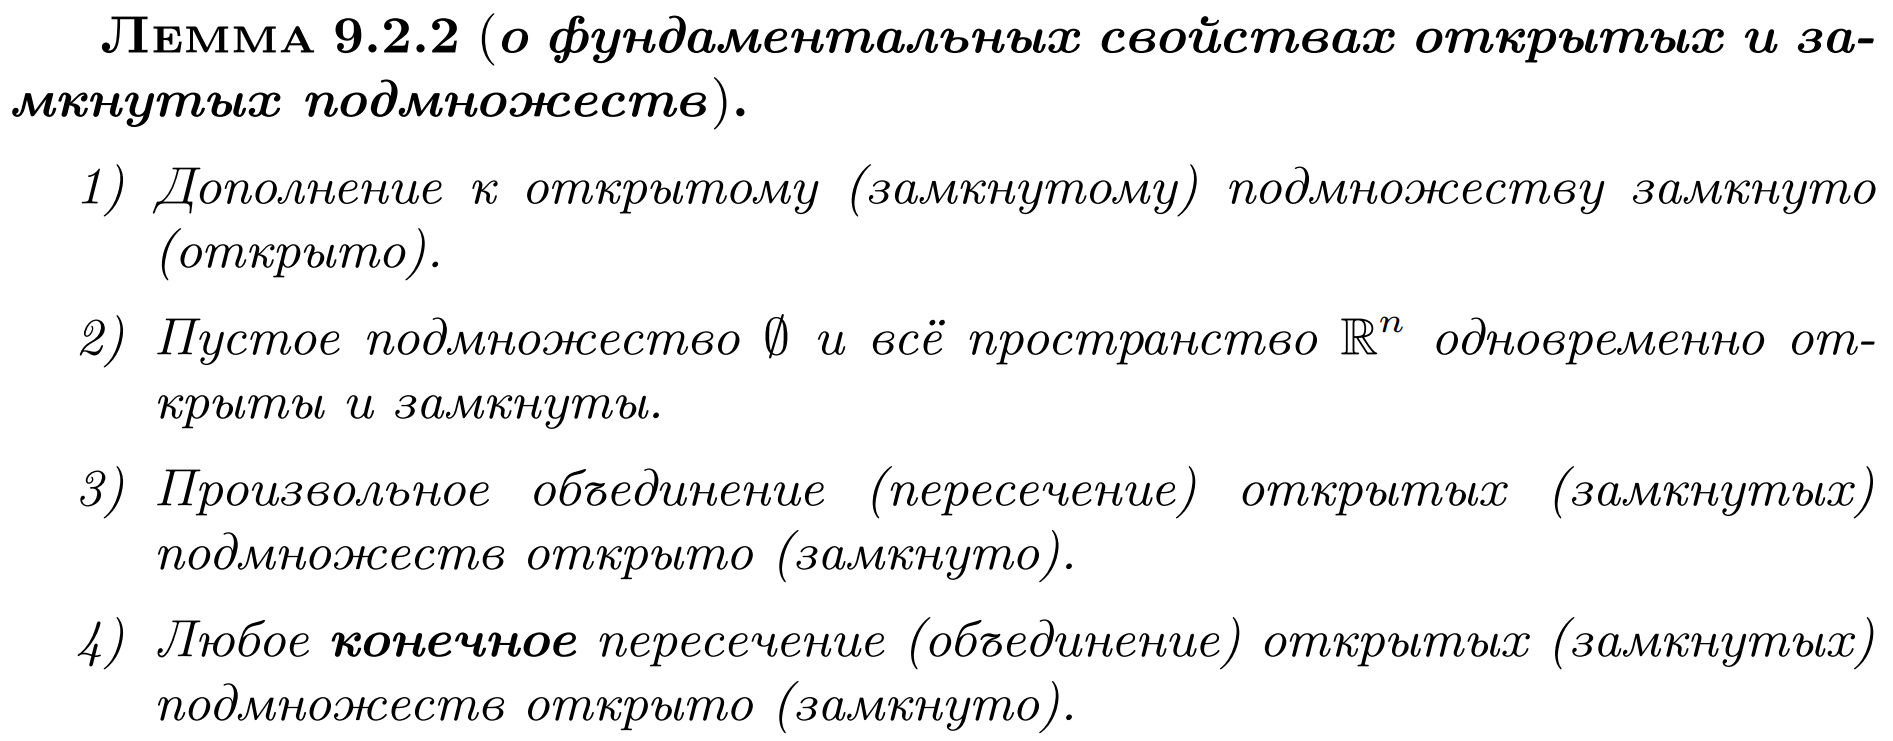
\includegraphics[width=\textwidth]{10.png}}
    \vspace{-1cm}
\end{figure}
\begin{figure}[h!]
    \centering
    \fbox{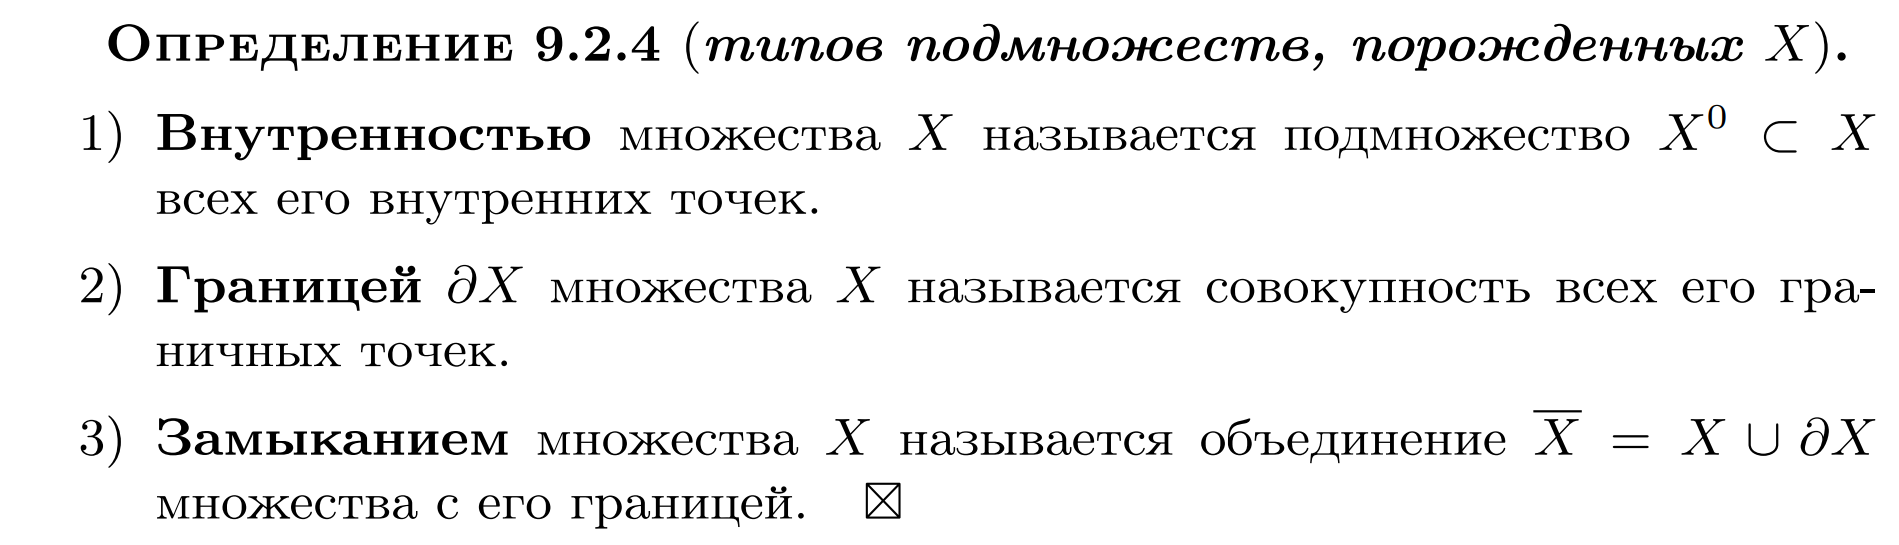
\includegraphics[width=\textwidth]{13.png}}
    \vspace{-1cm}
\end{figure}
\newpage\noindent
\bb{Summary}

\ii{Внутренняя точка} -- лежит в множестве вместе с окрестностью

\ii{Изолированная точка} -- существует проколотая окрестность, не содержащая точек множества

\ii{Предельная точка} -- точка, в любой проколотой окрестности которой есть точки из множества или есть последовательность Гейне, принадлежащая множеству

\ii{Граничная точка} -- любая окрестность содержит точки из множества и дополнения.

\ii{Точка прикосновения} -- в любой окрестности (не проколотой) есть точки из множества.

\ii{Открытое множество} -- все его точки внутренние.

\ii{Замкнутое множество} -- содержит все предельные точки, дополнение открыто, сожержит все граничные точки, точки прикосновения.

\ii{Область} -- открытое множество, точки которого можно соединить кривой (не обязательно гладкой), принадлежащей множеству.

\ii{Компакт} -- замкнутое множество, принадлежащее некоторой окрестности нуля.

\ii{Th} Пересечение конечного количества открытых множеств открыто.

\ii{Th} Объединение любого количества открытых множеств открыто.

\ii{Th} Аналогично с замкнутыми множествами.

\ii{Внутренность} -- множество всех внутренних точек.

\ii{Граница} -- множество всех граничных точек.

\ii{Замыкание} -- объединение множества с его границей.

\newpage\noindent
\section{\color{RedViolet}\textbf{Предел числовой функции нескольких переменных. Предел функции по множеству. Пределы по направлениям. Непрерывность функции нескольких переменных в точке и по множеству. Непрерывность сложной функции. Свойства функций, непрерывных на компакте — ограниченность, достижимость (точных) нижней и верхней граней, равномерная непрерывность. Теорема о промежуточных значениях функции, непрерывной в области.}}
\begin{figure}[h!]
    \centering
    
\includegraphics[width=\textwidth]{14.png}
    \vspace{-1cm}
\end{figure}
\begin{figure}[h!]
    \centering
    \fbox{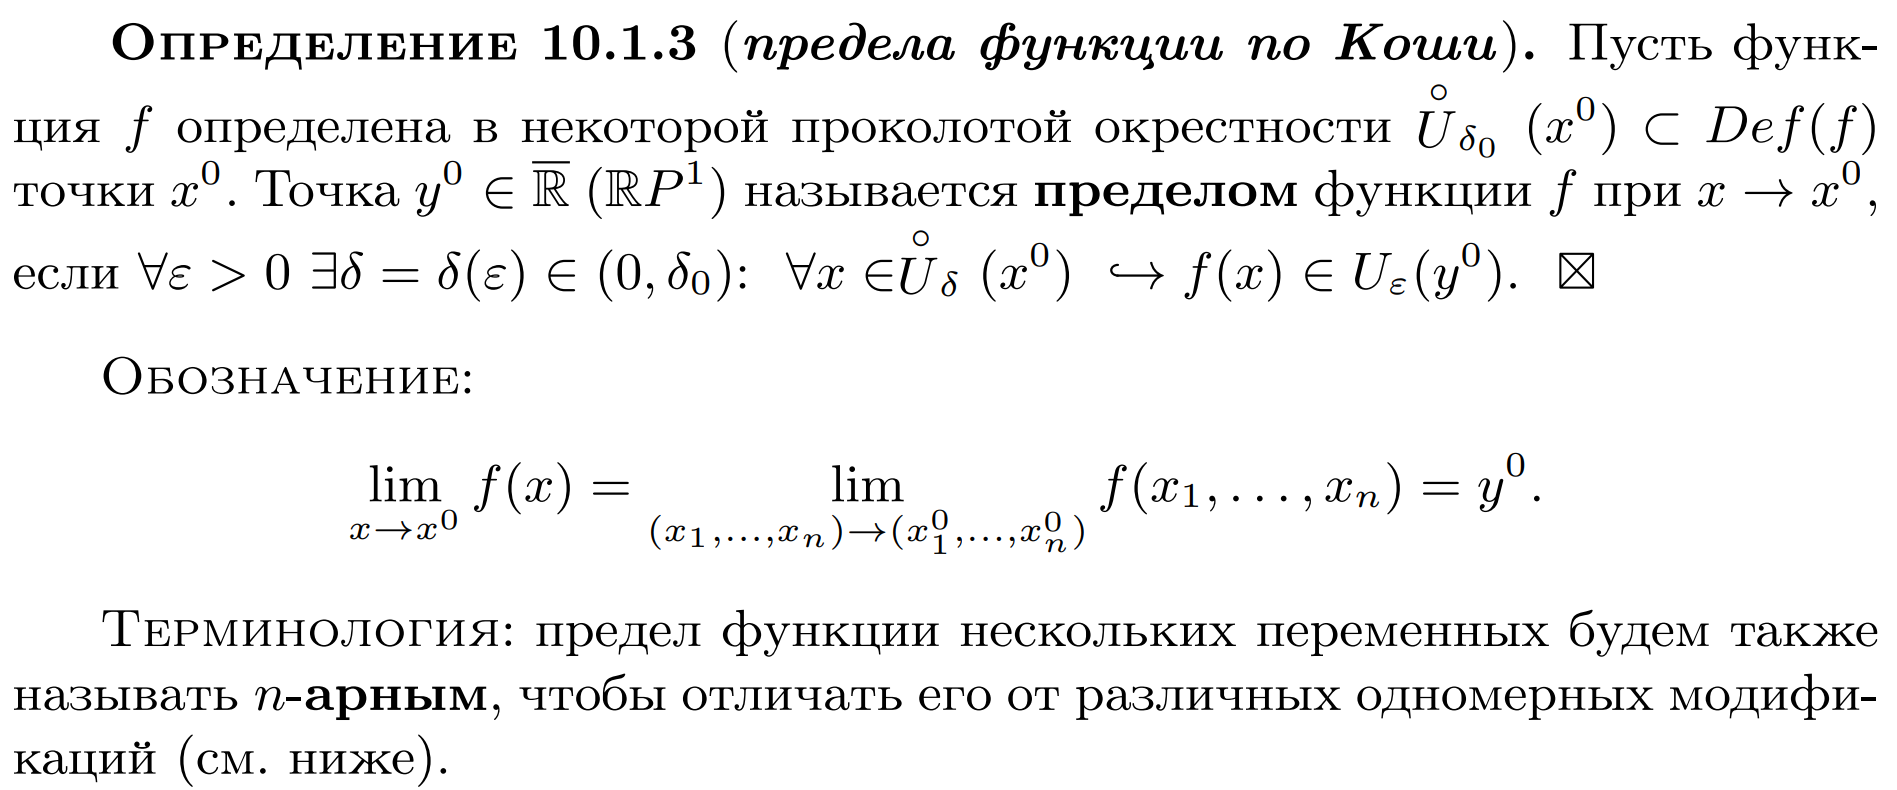
\includegraphics[width=\textwidth]{15.png}}
    \vspace{-1cm}
\end{figure}
\begin{figure}[h!]
    \centering
    \fbox{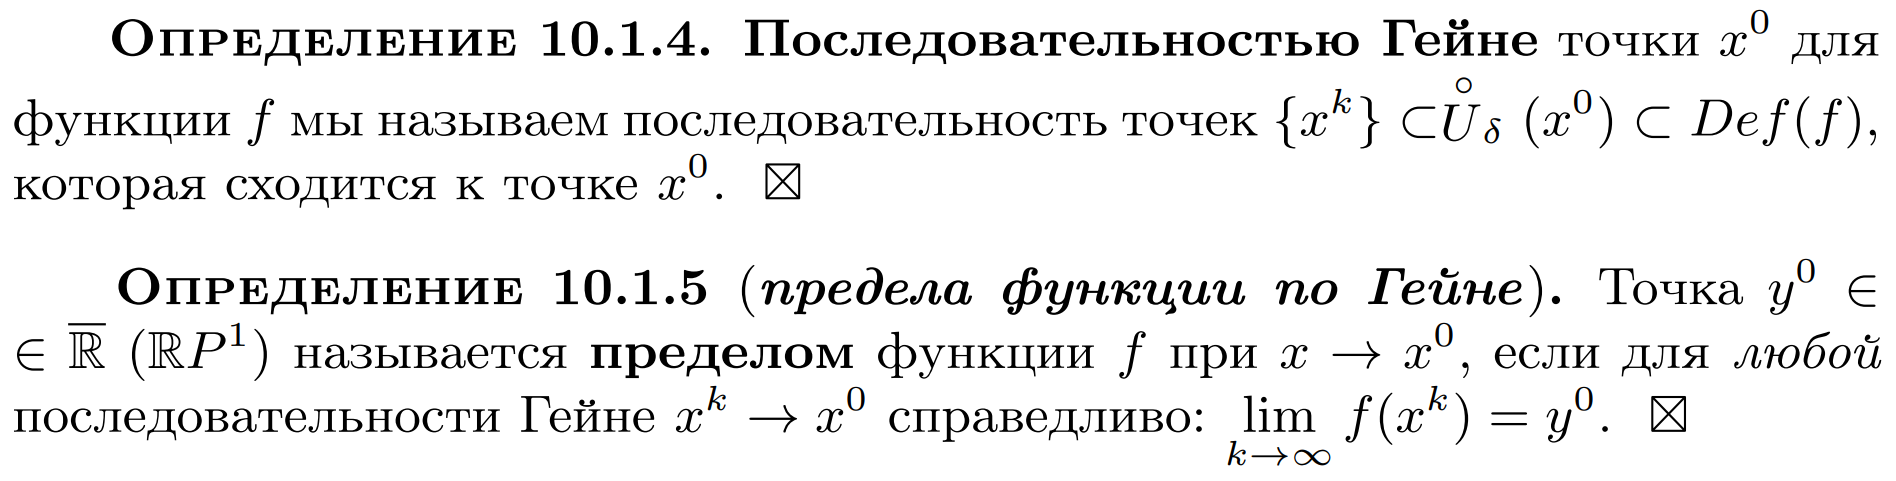
\includegraphics[width=\textwidth]{16.png}}
\end{figure}

{\bfseries\colorbox{lightgray}{Def}} \bb{Повторный предел} -- сначала берём предел по одной переменной, а потом по второй, рассматривая предел по первой как функцию.
$$\lim\limits_{y\to 0}\lim\limits_{x\to 0} \left( x+y \sin\frac{1}{x} \right) = \emptyset$$
$$\lim\limits_{x\to 0}\lim\limits_{y \to 0}\left( x + y \sin \frac{1}{x} \right) = 0 $$

\newpage
\begin{figure}[h!]
    \centering
    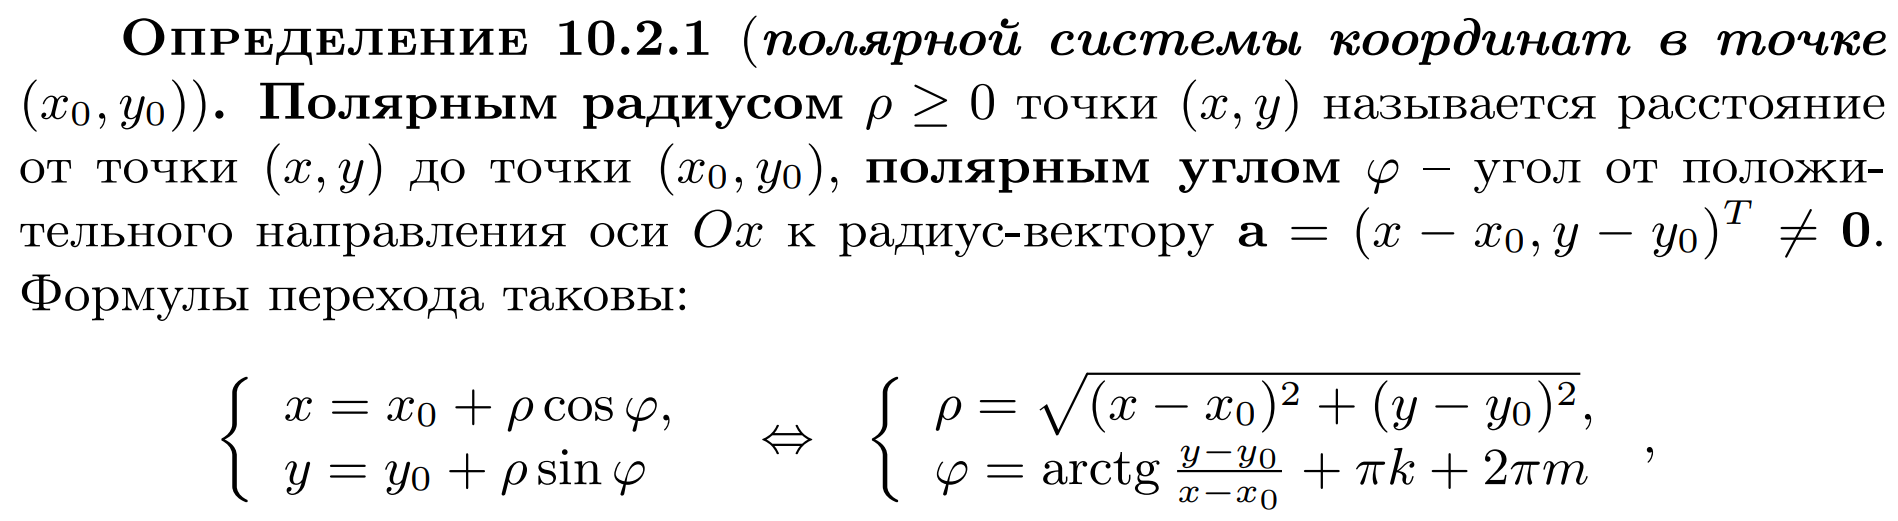
\includegraphics[width=\textwidth]{17.png}
    \vspace{-1cm}
\end{figure}
\begin{figure}[h!]
    \centering
    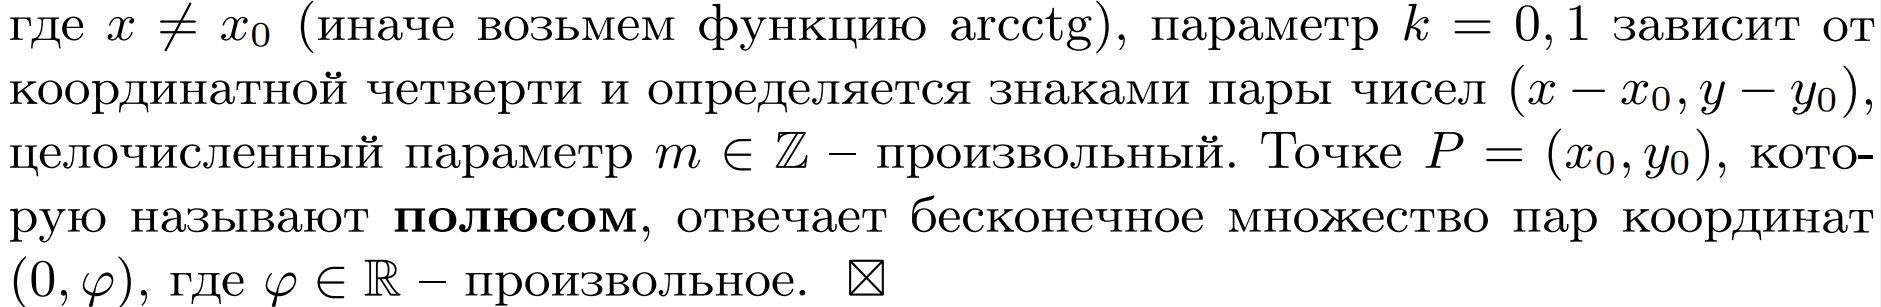
\includegraphics[width=\textwidth]{18.png}
    \vspace{-1cm}
\end{figure}
\begin{figure}[h!]
    \centering
    \fbox{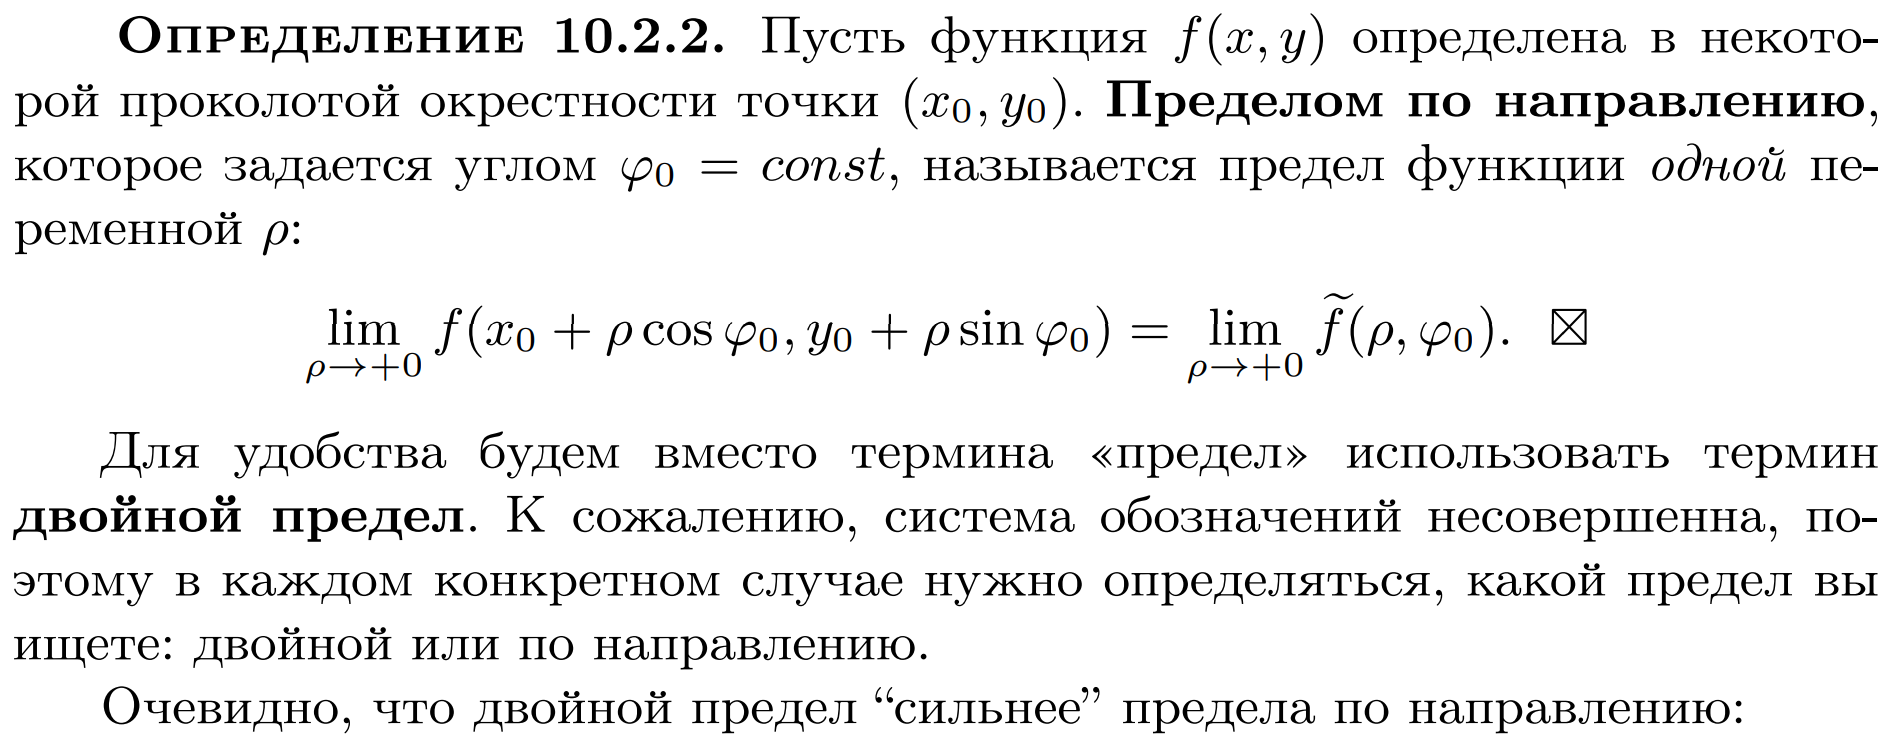
\includegraphics[width=\textwidth]{19.png}}
    \vspace{-1cm}
\end{figure}
\begin{figure}[h!]
    \centering
    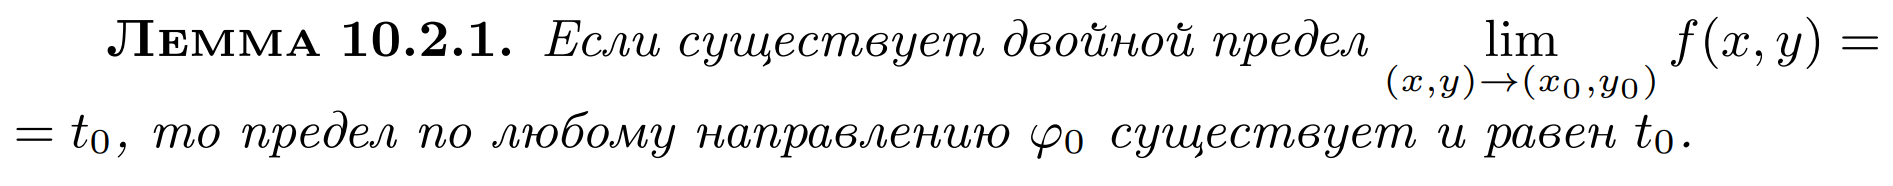
\includegraphics[width=\textwidth]{20.png}
    \vspace{-1cm}
\end{figure}
\begin{figure}[h!]
    \centering
    \fbox{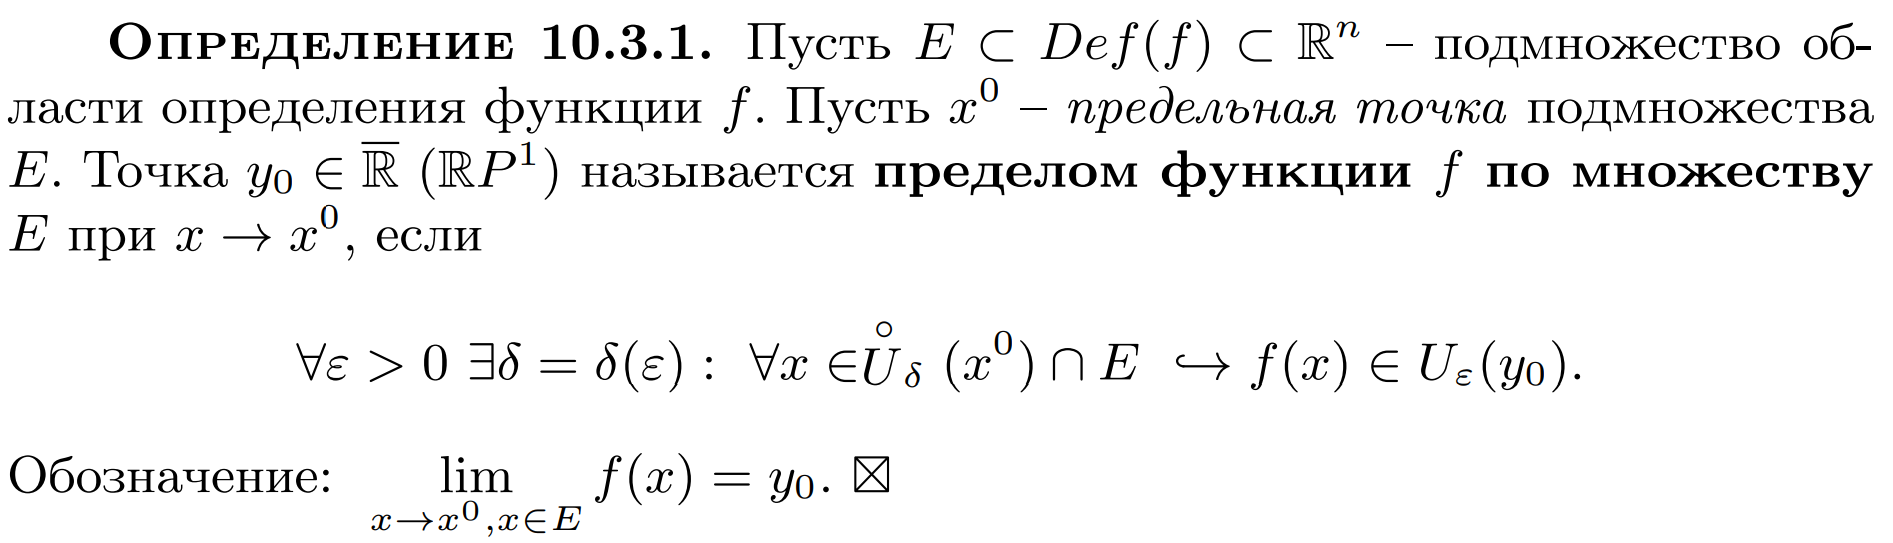
\includegraphics[width=\textwidth]{21.png}}
\end{figure}
Например, односторонние пределы функции одной переменной или предел по направлению функции нескольких переменных.
\newpage

{\bfseries\colorbox{lightgray}{Def}} (Скубачевский) Предел по направлению -- предел по множеству $E$, где $E$ -- луч.

\bb{Утв} $\exists \lim\limits_{x\to x^{(0)}} f(x) \Rightarrow$ в точке $x^{(0)}$ существует предел по всем направлениям, и они равны.

Обратное не верно. Пример: парабола, поднятая вверх на 1 для точки (0,0).
\begin{figure}[h!]
    \centering
    \fbox{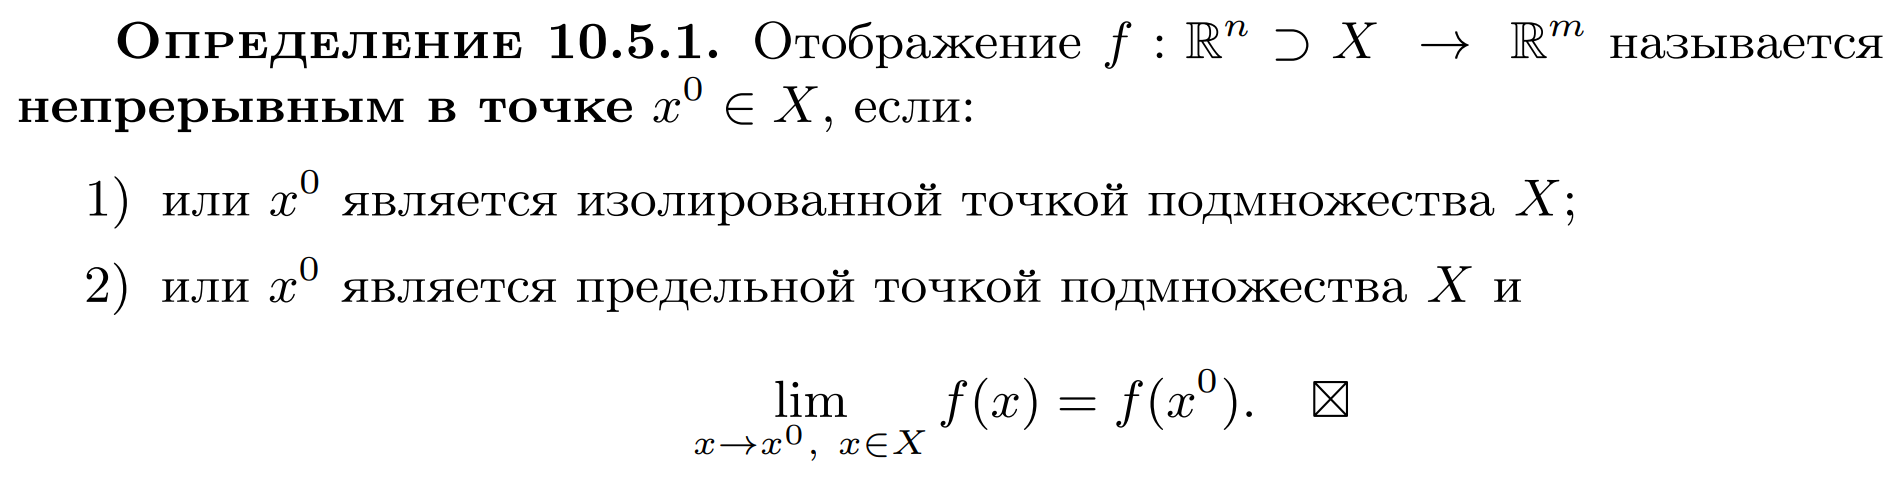
\includegraphics[width=\textwidth]{22.png}}
    \vspace{-1cm}
\end{figure}
\begin{figure}[h!]
    \centering
    
\includegraphics[width=\textwidth]{23.png}
    \vspace{-1cm}
\end{figure}
\begin{figure}[h!]
    \centering
    
\includegraphics[width=\textwidth]{24.png}
    \vspace{-1cm}
\end{figure}
\begin{figure}[h!]
    \centering
    
\includegraphics[width=\textwidth]{25.png}
    \vspace{-1cm}
\end{figure}
\begin{figure}[h!]
    \centering
    
\includegraphics[width=\textwidth]{26.png}
    \vspace{-1cm}
\end{figure}
\begin{figure}[h!]
    \centering
    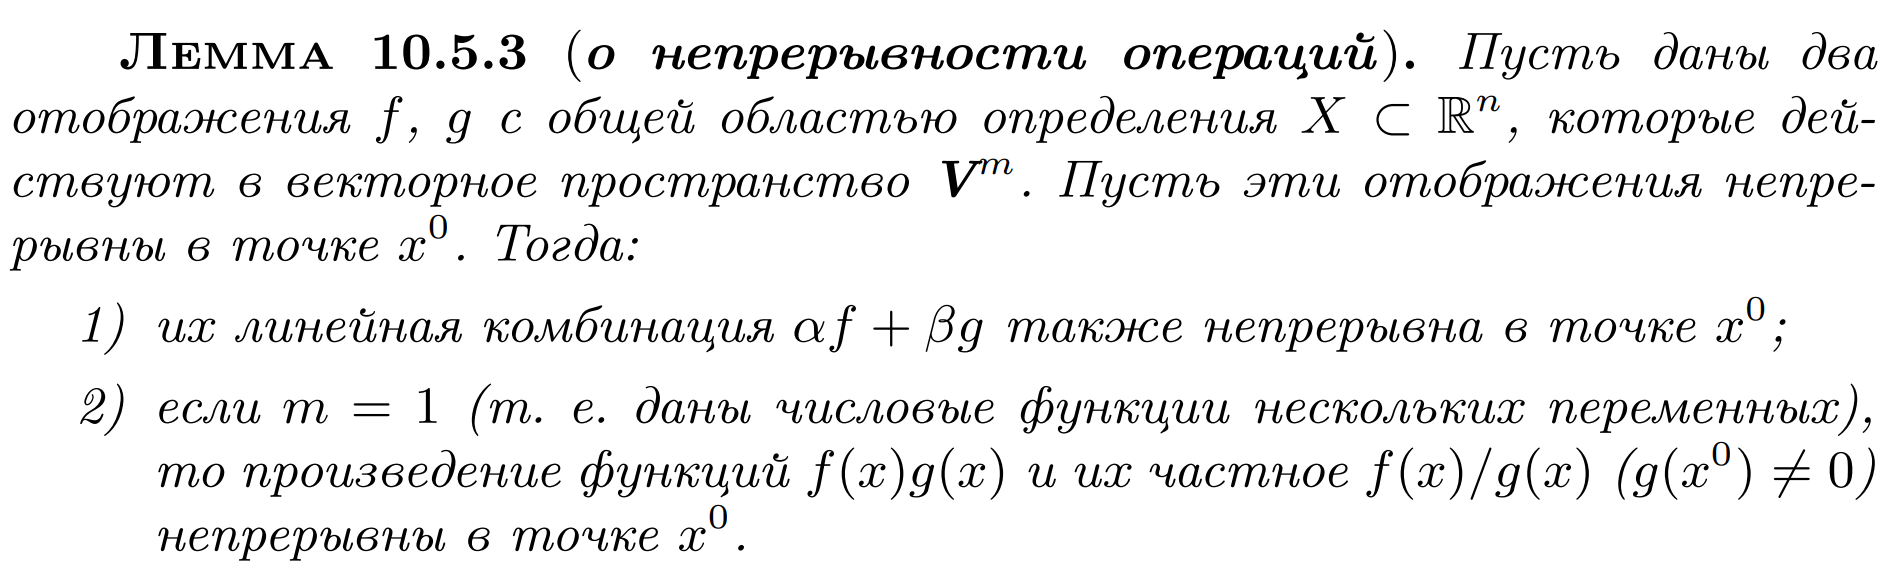
\includegraphics[width=\textwidth]{27.png}
    \vspace{-1cm}
\end{figure}
\newpage
\begin{figure}[h!]
    \centering
    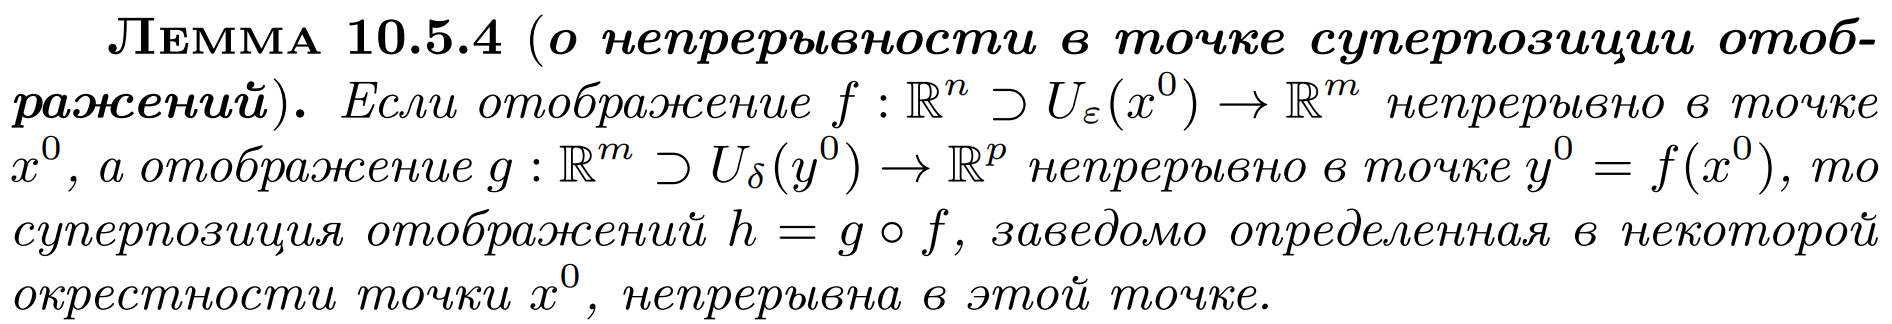
\includegraphics[width=\textwidth]{28.png}
    \vspace{-1cm}
\end{figure}
\begin{figure}[h!]
    \centering
    \fbox{
\includegraphics[width=\textwidth]{29.png}}
    \vspace{-1cm}
\end{figure}
\begin{figure}[h!]
    \centering
    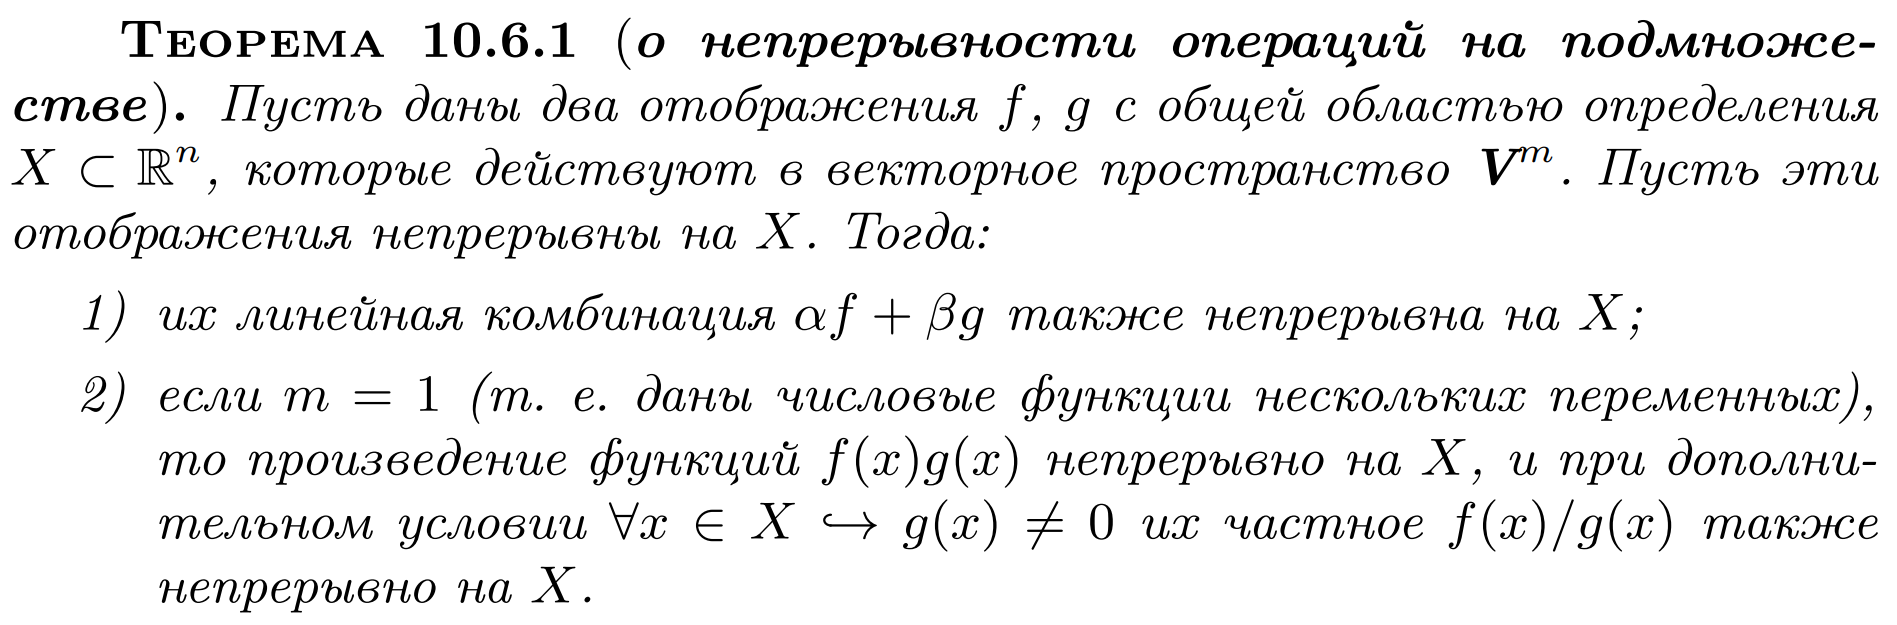
\includegraphics[width=\textwidth]{30.png}
    \vspace{-1cm}
\end{figure}
\begin{figure}[h!]
    \centering
    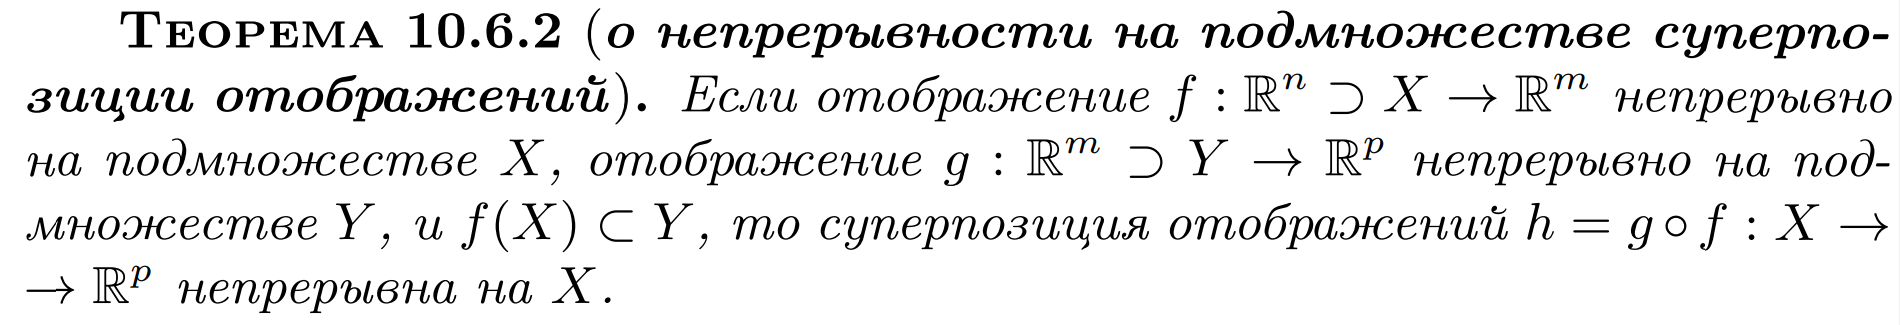
\includegraphics[width=\textwidth]{31.png}
    \vspace{-1cm}
\end{figure}
\newpage
\begin{figure}[h!]
    \centering
    
\includegraphics[width=\textwidth]{32.png}
    \vspace{-1cm}
\end{figure}

\newpage
\section{\color{RedViolet}\textbf{Частные производные функции нескольких переменных. Дифференцируемость функции в точке, дифференциал. Необходимые условия дифференцируемости, достаточные условия дифференцируемости функции нескольких переменных. Дифференцируемость сложной функции. Инвариантность формы дифференциала относительно замены переменных. Градиент и производная по направлению.}}

a
\newpage
\section{\color{RedViolet}\textbf{Неопределённые интегралы}}
\begin{itemize}
    \item \textbf{Замена переменной}
          \begin{equation*}
              \int\frac{dx}{\sqrt{e^x+1}} = \left|
              \begin{aligned}
                   & t = e^x-1    \\
                   & x = \ln(t+1)
              \end{aligned} \right| = \int\frac{dt}{\sqrt{t}(t+1)} = \left|
              \begin{aligned}
                   & u = \sqrt{t} \\
                   & t = u^2
              \end{aligned} \right| = \int\frac{2udu}{u(u^2+1)}
          \end{equation*}
    \item \textbf{Интегрирование по частям}
          \begin{equation*}
              \int u v'dx = uv - \int u' v dx
          \end{equation*}
    \item \textbf{Рациональные функции}
          $$\int\frac{P(x)}{Q(x)}dx $$
          \begin{enumerate}
              \item $\deg P \geq \deg Q \Rightarrow$ выделить целую часть
              \item Разложтить знаменатель на неприводимые множители
              \item Представить $P/Q$ в виде суммы
              \item Найти неопределённые коэффициенты
              \item Проинтегрировать каждое слагаемое
          \end{enumerate}
    \item \textbf{Метод Остроградского}
          $$ \int \frac{P}{Q}dx = \frac{P_1}{Q_1} + \int \frac{P_2}{Q_2}dx$$
          $Q_2$ произведение всех неприводимых множителей $Q$, $Q_1 = Q/Q_2$
          $$ \int\frac{x^3+x^2-4x+1}{(x^2+1)^2}dx = \frac{Ax + B}{x^2+1} + \int\frac{Cx + D}{x^2+1} $$
          Дальше дифференцируем и находим коэффициенты.
    \item \textbf{Иррациональности}
          \begin{enumerate}
              \item $R(\alpha,\beta, \gamma,\ldots) = {P(\alpha, \beta, \gamma, \ldots)}/{Q(\alpha, \beta, \gamma, \ldots)} $
                    \begin{multline*}
                        \int R\left(x, \left(\frac{ax + b}{cx+d}\right)^{p_1/q_1}, \left(\frac{ax + b}{cx+ d}\right)^{p_2/1_2}, \ldots \right)dx = \\ = \left|
                        \begin{aligned}
                             & t^N = \frac{ax+b}{cx+d}       \\
                             & N = \x{НОК}(q_1, q_2, \ldots)
                        \end{aligned} \right| = \ldots
                    \end{multline*}
              \item Дифференциальный бином
                    $$ \int x^m (ax^n+b)^pdx $$
                    \begin{enumerate}
                        \item $p$ -- целое $\Rightarrow$ $x = t^N, \; N = \x{НОК}(\x{зн}(m), \x{зн}(n))$
                        \item $(m+1)/{n}$ -- целое $\Rightarrow$ $ax^n+b = t^s, \; s=\x{зн}(p)$
                        \item ${(m+1)}/{n}+p$ -- целое $\Rightarrow$ $a + b x^{-n} = t^s, \; s=\x{зн}(p)$
                        \item В остальных случаях интеграл не берётся.
                    \end{enumerate}
              \item Подстановки Эйлера
                    $$ \int R\left(x, \sqrt{ax^2+bx+c}\right)dx $$
                    \begin{equation*}
                        \sqrt{ax^2+bx+c} = \left\{
                        \begin{aligned}
                             & \pm \sqrt{a}x \pm t, \; a > 0 \\
                             & \pm xt \pm \sqrt{c}, \; c > 0 \\
                             & (x-x_{1,2})t
                        \end{aligned}
                        \right.
                    \end{equation*}
              \item $P(x, \sqrt{p})/Q(x, \sqrt{p})$
                    $$ \frac{P(x, \sqrt{p})}{Q(x, \sqrt{p})} = R_1(x) + R_2(x) \frac{1}{\sqrt{p}} $$
                    $$ \int\frac{\widetilde{p}(x)}{\sqrt{p}}dx = \widetilde{Q}(x)\sqrt{p} + \lambda\int\frac{1}{\sqrt{p}}dx $$
          \end{enumerate}
    \item \textbf{Тригонометрия}
          \begin{enumerate}
              \item $\int (\sin^nx \cdot \cos^m x ) dx  = |m \x{--нечёт}| = \int (\sin^nx\cdot \cos^{2k}x)d(\sin x)$
              \item $$\int \frac{P(\sin x, \cos x)}{Q(\sin x, \cos x)} dx, \quad P,Q\x{-- однородные, } \deg Q = \deg P + 2$$
                    Поделить обе части на $\cos^2x$, прератив в тангенсы.
              \item $\deg Q - \deg P = 2k \Rightarrow $ домножить на $(\cos^2x + \sin^2 x)$
              \item Сделать степени чётными, увеличив угол в два раза.
                    \begin{equation*}
                        \int \frac{1- \sin x + \cos x}{1+ \sin x - \cos x} dx = \left|
                        \begin{aligned}
                             & x = 2t       \\
                             & u = \tg t    \\
                             & u = \tg(x/2)
                        \end{aligned} \right| = \bigintsss{\ddfrac{1 - \frac{2u}{1+u^2} + \frac{1 - u^2}{1 + u^2}}{1 + \ddfrac{2u}{1+u^2} - \frac{1-u^2}{1 + u^2}}\frac{2 du}{1 + u^2}}
                    \end{equation*}
          \end{enumerate}
\end{itemize}



\end{document}
